\documentclass[12pt]{article}
\usepackage[utf8]{inputenc}
\usepackage[russian]{babel}
\usepackage{amsmath}
\usepackage[pdf]{graphviz}
\usepackage{listings}
\usepackage{color}
\usepackage{braket}

\definecolor{dkgreen}{rgb}{0,0.6,0}
\definecolor{gray}{rgb}{0.5,0.5,0.5}
\definecolor{mauve}{rgb}{0.58,0,0.82}

\lstset{frame=tb,
  language=C++,
  aboveskip=3mm,
  belowskip=3mm,
  showstringspaces=false,
  columns=flexible,
  basicstyle={\small\ttfamily},
  numbers=none,
  numberstyle=\tiny\color{gray},
  keywordstyle=\color{blue},
  commentstyle=\color{dkgreen},
  stringstyle=\color{mauve},
  breaklines=true,
  breakatwhitespace=true,
  tabsize=3
}

\begin{document}
	\title{Домашняя работа по ТМВ №3}
	\author{Корнев Илья А-13б-19}
	\date{}
	\maketitle
	\setlength{\footskip}{60pt}
	\section*{Задание 2.1 Работа с числами}
	1. Сложение двух унарных чисел\\
	\indent На вход подаются унарные числа разделенные символом '+', можно поступить по хитрому:\\
	\indent Заменим + на 1 и затем удалим последнюю единицу.
	\begin{lstlisting}
		input: '111+11'
 		blank: ' '
  		start state: replace_plus
  		table:
    		replace_plus:
      			1: R
      			'+': {write: 1, R: find_end}
    		find_end:
      			1: R
      			' ': {L : delete_last_one}
    		delete_last_one:
      			1: {write : ' ', L: done}
    		done:
	\end{lstlisting}
	2. Умножение двух унарных чисел\\
	\indent Ставим знак равенства как разделителбь между ответом и множителями\\
	\indent Переносим первый множитель за знак равенства столько раз, сколько единиц во втором множителе\\
	\indent Затем удаляем все, что не относится к ответу
	\begin{lstlisting}
	input: '11*11'
	blank: ' '
	start state: put_eq
	table:
	  put_eq: 
	    [1, '*']: R
	    ' ': {write: =, L: left}
	  left:
	    [1, '*']: L
	    ' ': {R: start_mul}
	  start_mul:
	    1: {write: a, R: to_second}
	    a: R
	    '*': {L: to_left_end}
	  to_second:
	    1: R
	    '*': {R: second}
	  second:
	    a: R
	    1: {write: a, R: carry_to_answer}
	    =: {L: restore_second}
	  carry_to_answer:
	    [1, =]: R
	    ' ': {write: 1, L: back_to_second}
	  back_to_second:
	    [1, =]: L
	    a: {R: second}
	  restore_second:
	    a: {write: 1, L}
	    '*': {L: to_first}
	  to_first:
	    1: L
	    a: {R: start_mul}
	  to_left_end:
	    a: L
	    ' ': {R: del_all}
	  del_all:
	    [1, '*', a]: {write: ' ', R: del_all}
	    =: {write: ' ', R: done}
	  done:
	\end{lstlisting}
	
	\section*{Задание 2.2 Работа с символами}
	1. Принадлежность к языку $L = \{0^n1^n2^n\}$\\
	\indent Поочередно заменяем 0, 1 и 2 на временный символ 'a', затем возвращаем каретку назад в начало слова и повторяем процесс.\\
	\indent Если при выполнении первого шага с прасопзнованием нуля мы находим пустой символ, то переходим к состоянию успеха: удаляем всю строку и печатаем сивол 's'.\\
	\indent Если в посреди последовательности из 0, 1 или 2 мы находим другой символ (например $0001\boldsymbol{0}1222$), то переходим в состояние неуспеха: удаляем всю строку и печатаем символ 'f'.
	\begin{lstlisting}
	input: '0010122'
	blank: ' '
	start state: consume_0
	table:
	  consume_0:
	    ' ': {L: success}
	    0: {write: a, R: consume_1}
	    [1, 2]: {R: fail}
	    a: R
	  consume_1:
	    [0, a]: R
	    1: {write: a, R: consume_2}
	    [2, ' ']: {L: fail}
	  consume_2:
	    [1, a]: R
	    2: {write: a, L: back_to_start}
	    [0,' ']: {L: fail}
	  back_to_start:
	    [a, 0, 1, 2]: L
	    ' ': {R: consume_0}
	  success:
	    a: {write: ' ', L}
	    ' ': {write: s, R: done}
	  fail:
	    [a, 0, 1, 2]: R
	    ' ': {L: del}
	  del:
	    [a, 0, 1, 2]: {write: ' ', L}
	    ' ': {write: f, R: done}
	  done:
	\end{lstlisting}
	2. Проверка соблюдения правильности скобок (минимум 3 вида скобок):
	\indent Находим первую правую скобку\\
	\indent Затем проверяем предшествующую ей, если она такого же типа, то заменяем обе на временный символ 'a' и переходим в начальное состояние, иначе переходим в состояние неуспеха: удаляем строку и печатаем символ 'f'\\
	\indent Если переходя обратно в начальное состояние мы находим конец строки, то переходи в состояние успеха: печатаем символ 's' и удаляем остальную строку.
	\begin{lstlisting}
	input: '([({})])({[]}){}'
	blank: ' '
	start state: left
	table:
	  left:
	    ' ': {L: to_begin}
	    a: R
	    ['(','[','{']: {R: left_p}
	    ')': {write: a, L: right_p}
	    ']': {write: a, L: right_br}
	    '}': {write: a, L: right_curl}
	  left_p:
	    ' ': {L: fail}
	    a: R
	    ['(','[','{']: {R: left_p}
	    ')': {write: a, L: right_p}
	    ']': {write: a, L: right_br}
	    '}': {write: a, L: right_curl}
	  right_p:
	    a: L
	    '(': {write: a, L: try_left}
	    ['{', '[']: {write: a, L: fail}
	    ' ': {R: fail}
	  right_br:
	    a: L
	    '[': {write: a, L: try_left}
	    ['{', '(']: {write: a, L: fail}
	    ' ': {R: fail}
	  right_curl:
	    a: L
	    '{': {write: a, L: try_left}
	    ['(', '[']: {write: a, L: fail}
	    ' ': {R: fail}
	  try_left:
	    ' ': {R: left}
	    [a, '{', '[', '(']: {R: back_to_left}
	  back_to_left:
	    a: {L: left}
	    ' ': L
	  to_begin:
	    ' ': {R: success}
	    a: L
	    ['{', '[', '(']: {L: try_left}
	  success:
	    [a, ' ']: {write: s, R: to_end}
	  to_end:
	    [a, '{', '[', '(', '}', ']', ')']: R
	    ' ': {L: clear}
	  clear: 
	    [a, '{', '[', '(', '}', ']', ')']: {write: ' ', L}
	    d: L
	    ' ': {R: done}
	  fail:
	    [a, '{', '[', '(', '}', ']', ')', ' ']: {R: to_end}
	  done:
	    ' ': {write: f, R: back_to_left}
	\end{lstlisting}
	3. Поиск минимального по длине слова в строке (слова состоят из символов 1 и 0 и разделены пробелом)
	\indent Обрабатываем первые два слова, сравниваем их длину, заменяя 0 и 1 на временные символы (0=a, 1=b), и затем если в состоянии для проверки второго слова мы находим пустую строку, то второе меньше, иначе первое меньше.\\
	\indent Если первое слово длинее, стираем его и востанавливаем его из временных символов.\\
	\indent Если второе оказалось больше, копируем первое на место второго и удаляем то, что осталось от второго.
	\begin{lstlisting}
	input: '1010 010 01 000'
	blank: ' '
	start state: first_word
	table:
	  first_word:
	    0: {write: a, R: to_second}
	    1: {write: b, R: to_second}
	    [a, b]: R
	    ' ': {L: first_is_smaller}
	  to_second:
	    [0, 1]: R
	    ' ': {R: second_word}
	  second_word:
	    ' ': {L: one_left}
	    0: {write: a, L: to_first}
	    1: {write: b, L: to_first}
	    [a, b]: {R: second_not_null}
	  second_not_null:
	    [a, b]: R
	    0: {write: a, L: to_first}
	    1: {write: b, L: to_first}
	    ' ': {L: second_is_smaller}
	  to_first:
	    [a, b]: L
	    ' ': {L: to_begin_first}
	  to_begin_first:
	    [0, 1, a, b]: L
	    ' ': {R: first_word}
	  one_left:
	    ' ': {L: restore_and_exit}
	  restore_and_exit:
	    a: {write: 0, L}
	    b: {write: 1, L}
	    [0, 1]: L
	    ' ': {R: done}
	  first_is_smaller:
	    [a, b]: L
	    ' ': {R: restore_first}
	  restore_first:
	    a: {write: 0, R}
	    b: {write: 1, R}
	    ' ': {R: cut_second}
	  cut_second:
	    [a, b, 0, 1]: {write: a, R}
	    ' ': {L: return_and_copy}
	  return_and_copy:
	    a: L
	    ' ': {L: copy_first}
	  copy_first:
	    [a, b]: L
	    0: {write: a, R: carry0}
	    1: {write: b, R: carry1}
	    ' ': {R: delete_to_word}
	  carry0:
	    [a, b]: R
	    ' ': {R: carry0_in_second}
	  carry0_in_second:
	    a: R
	    [0, 1, ' ']: {L: set0_and_return}
	  set0_and_return:
	    a: {write: 0, L: return_and_copy}
	    ' ': {L: return_and_copy}
	  carry1:
	    [a, b]: R
	    ' ': {R: carry1_in_second}
	  carry1_in_second:
	    a: R
	    [0, 1, ' ']: {L: set1_and_return}
	  set1_and_return:
	    a: {write: 1, L: return_and_copy}
	    ' ': {L: return_and_copy}
	  delete_to_word:
	    [a, b]: {write: ' ', R}
	    [0, 1]: {L: to_begin_first}
	    ' ': {R: delete_to_word_in_sec}
	  delete_to_word_in_sec:
	    [a, b]: {write: ' ', R}
	    [0, 1]: {L: to_begin_first}
	    ' ': {R: done}
	  second_is_smaller:
	    [a, b]: L
	    ' ': {L: to_begin_first_and_del}
	  to_begin_first_and_del:
	    [0, 1, a, b]: L
	    ' ': {R: delete_first}
	  delete_first:
	    [0, 1, a, b]: {write: ' ', R}
	    ' ': {R: restore_second}
	  restore_second:
	    a: {write: 0, R}
	    b: {write: 1, R}
	    ' ': {L: to_begin_first}
	  done:
	\end{lstlisting}
	
	\section*{Задание 3. Квантовые вычисления}
	3.1 Генерация суперпозиций\\
	\indent Дано $N$ кубитов ($1 \le N \le 8$) в нулевом состоянии $\Ket{0\dots0}$. Также дана некоторая последовательность битов, которое задаёт ненулевое базисное состояние размера $N$. Задача получить суперпозицию нулевого состояния и заданного.

	$$\Ket{S} = \frac{1}{\sqrt2}(\Ket{0\dots0} +\Ket{\psi})$$

	То есть требуется реализовать операцию, которая принимает на вход:

	\begin{enumerate}
    		\item Массив кубитов $q_s$
   		 \item Массив битов $bits$ описывающих некоторое состояние $\Ket{\psi}$. Это массив имеет тот же самый размер, что и $qs$. Первый элемент этого массива равен $1$.
	\end{enumerate}
	\indent По условию первым различным кубитом является самый первый, для начала применим к нему оператор адамара $H$, затем будем запутывать его со всеми единичными кубитами второго вектора с помощью CNOT.\\
	Частный случай:
		$$\Ket{S} = \frac{1}{\sqrt{2}}(\Ket{000} + \Ket{111})$$
	\begin{center}
		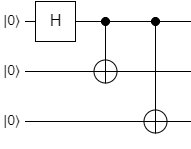
\includegraphics[scale=1]{curcuit.png}
	\end{center}
	\begin{lstlisting}
	namespace Solution
	 {
	    open Microsoft.Quantum.Primitive;
	    open Microsoft.Quantum.Canon;
	    
	    operation Solve(qs: Qubit[], bits: Bool[]) : () 
	    {
	        body 
	        { 
	            H(qs[0]);
	            for (i in 1..Length(qs) - 1)
	             {
	                if (bits[i])
	                 {
	                    CNOT(qs[0], qs[i]); 
	                } 
	            }                  
	        }
	    }
	}
\end{lstlisting}
	
	3.2 Различие состояний 1\\
	Дано $N$ кубитов ($1 \le N \le 8$), которые могут быть в одном из двух состояний:

	$$\Ket{GHZ} = \frac{1}{\sqrt2}(\Ket{0\dots0} +\Ket{1\dots1})$$
	$$\Ket{W} = \frac{1}{\sqrt N}(\Ket{10\dots00}+\Ket{01\dots00} + \dots +\Ket{00\dots01})$$

	Требуется выполнить необходимые преобразования, чтобы точно различить эти два состояния. Возвращать $0$, если первое состояние и 1, если второе.\\
	
	Эти два состояния легко различимы, достаточно лишь измерить кубиты: если они были в первом состоянии, при измерении получим либо N нулей либо N единиц, иначе только равно одну единицу.\\
	Частный случай для $N=3$
	$$\Ket{GHZ} = \frac{1}{\sqrt{2}}(\Ket{000} +\Ket{111})$$
	$$\Ket{W} = \frac{1}{\sqrt{3}}(\Ket{100}+\Ket{010} + \Ket{001})$$
	
	\begin{lstlisting}
	namespace Solution 
	{
	    open Microsoft.Quantum.Primitive;
	    open Microsoft.Quantum.Canon;
	    operation Solve(qs: Qubit[]) : Int 
	    {
	        body
	        {   
	            mutable countOnes = 0;
	            for (q in qs)
	            {
	                if (M(q) == One) 
	                { 
	                    set countOnes = countOnes + 1; 
	                }
	            }
	            
	            if(countOnes == Length(qs) or countOnes == 0)
	            {
	            	return 0;
	            }
	            else
	            {
	            	return 1;
	            }
	    }
	}
	\end{lstlisting}
	3.3 Различие состояний 2\\
	Дано $2$ кубита, которые могут быть в одном из двух состояний:

	$$\Ket{S_0} = \frac{1}{2}(\Ket{00} + \Ket{01} + \Ket{10} + \Ket{11})$$
	$$\Ket{S_1} = \frac{1}{2}(\Ket{00} - \Ket{01} + \Ket{10} - \Ket{11})$$
	$$\Ket{S_2} = \frac{1}{2}(\Ket{00} + \Ket{01} - \Ket{10} - \Ket{11})$$
	$$\Ket{S_3} = \frac{1}{2}(\Ket{00} - \Ket{01} - \Ket{10} + \Ket{11})$$


	Требуется выполнить необходимые преобразования, чтобы точно различить эти четыре состояния. Возвращать требуется индекс состояния (от $0$ до $3$). 
	\\\\
	Для различия данных состояний применим к каждому кубиту оператор $H^{\otimes2}$:
	$$
	H^{\otimes2} = \frac{1}{2}
	\begin{pmatrix}
		1 & 1 & 1 & 1\\
		1 & -1 & 1 & -1 \\
		1 & 1 & -1 & -1\\
		1 & -1 & -1 & 1\\
	\end{pmatrix}
	$$
	Если записать наши 4 состояния в векторной форме:
	$$
	\Ket{S_0} = \frac{1}{2} \begin{pmatrix} 1\\1\\1\\1\end{pmatrix},
	\Ket{S_1} = \frac{1}{2} \begin{pmatrix} 1\\-1\\1\\-1\end{pmatrix},
	\Ket{S_2} = \frac{1}{2} \begin{pmatrix} 1\\1\\-1\\-1\end{pmatrix},
	\Ket{S_3} = \frac{1}{2} \begin{pmatrix} 1\\-1\\-1\\1\end{pmatrix}
	$$
	То видно, что после применения оператора Адамара мы получаем 4 легко-различимых вектора:
	$$
	H^{\otimes2} \Ket{S_0} = \begin{pmatrix} 1\\0\\0\\0\end{pmatrix} = \Ket{00},
	H^{\otimes2} \Ket{S_1} = \begin{pmatrix} 0\\1\\0\\0\end{pmatrix} = \Ket{01},
	$$
	$$
	H^{\otimes2} \Ket{S_2} = \begin{pmatrix} 0\\0\\1\\0\end{pmatrix} = \Ket{10},
	H^{\otimes2} \Ket{S_3} = \begin{pmatrix} 0\\0\\0\\1\end{pmatrix} = \Ket{11}
	$$
	Затем достаточно измерить кубиты:
	
	\begin{lstlisting}
	namespace Solution
	{
	    open Microsoft.Quantum.Primitive;
	    open Microsoft.Quantum.Canon;
	    operation Solve (qs : Qubit[]) : Int 
	    {
	        body 
	        {
	            H(qs[0]);
	            H(qs[1]);
	            if (M(qs[0]) == Zero) 
	            {
	                if (M(qs[1]) == Zero) 
	                {
	                    return 0;
	                }
	                else 
	                {
	                    return 1;
	                }
	            }
	            else 
	            {
	                if (M(qs[1]) == Zero) 
	                {
	                    return 2;
	                }
	                else 
	                {
	                    return 3;
	                }
	            }
	        }
	    }
	}
\end{lstlisting}

\end{document}